% Drawing 80/01-4 -- folder 80, batch 01, archive page 9 (PDF page 10).
% Transcription: au-dessous de la grande figure, à gauche, deux petits hexagones de sommets $C'$, $A$, $B'$, $C$, $A'$, $B$ (dans cet ordre) : le premier, à diagonales épaisses, est entièrement couvert d'un gribouillis ; le second porte un trait épais du côté $C'A$ vers l'intérieur, prolongé au crayon vers $A'$, une diagonale au crayon de $C'$ à $C$, un trait de $B$ à $B'$ marqué de deux points, et un « $B$ » à l'intérieur
% Kind: hexagon with diagonals (a second one struck). Method 2 (schematic redraw from the facsimile). Status: partial.
% Notes: Two ink hexagons. The upper one is scribbled over (struck) and is not drawn. The lower one: six vertices labelled C', A, B', C, A', B clockwise from the top left, sides heavy; a heavy stroke from the middle of side C'A to an inner point, continued in pencil towards A'; a pencil diagonal from C' through that inner point to C; a line from B to B' carrying two heavy dots; the letter B inside. Left out: the small stroke with a blot to the right of the hexagon. Still differs: the inner strokes are a reading of a small free-hand figure (which strokes are meant as the three long diagonals is not certain). Redrawn 2026-11-12 (issue 128): to check again.
% Coordinates: 1 unit = 1 mm = 1/100 of the crop width (bbox in page fractions: [0.17, 0.635, 0.45, 0.83]).
% Redrawn by Claude (claude-fable-5-2), issue #128, 2026-11-12; not checked by a human; not compiled (no TeX in the session).
% Rights: reproduces part of the work -- behind RENDER_TRANSCRIPTS, never published by itself.
\documentclass[tikz,border=3pt]{standalone}
\usepackage{amsmath,amssymb}
\usetikzlibrary{patterns,arrows.meta}
\tikzset{pencil/.style={black!45}, struck/.style={black!35}, mpt/.style={circle,draw,inner sep=1.3pt}, pt/.style={circle,fill,inner sep=0.9pt}, opt/.style={circle,draw,fill=white,inner sep=1.1pt}}
\begin{document}
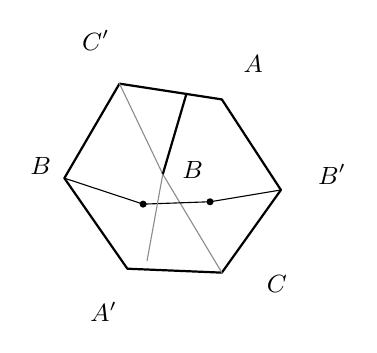
\begin{tikzpicture}[x=1mm,y=1mm,line cap=round,line join=round,font=\scriptsize]
\draw[thick] (17,-54) -- (30,-56) -- (37.5,-67.5) -- (30,-78) -- (18,-77.5) -- (10,-66) -- (17,-54);
\draw[pencil] (17,-54) -- (22.5,-65.5) -- (30,-78);
\draw (10,-66) -- (20,-69.3) -- (28.5,-69) -- (37.5,-67.5);
\draw[thick] (25.5,-55.3) -- (22.5,-65.5);
\draw[pencil] (22.5,-65.5) -- (20.5,-76.5);
\node[pt] at (20,-69.3) {};
\node[pt] at (28.5,-69) {};
\node[inner sep=1pt] at (14,-48.5) {\small $C'$};
\node[inner sep=1pt] at (34,-51.5) {\small $A$};
\node[inner sep=1pt] at (44,-65.5) {\small $B'$};
\node[inner sep=1pt] at (37,-79.5) {\small $C$};
\node[inner sep=1pt] at (15,-83) {\small $A'$};
\node[inner sep=1pt] at (7,-64.5) {\small $B$};
\node[inner sep=1pt] at (26.3,-65) {\small $B$};
\end{tikzpicture}
\end{document}
